% !TeX program = xelatex
% !TeX encoding = UTF-8
\documentclass[runningheads,a4paper]{llncs}
\usepackage{iftex}
\ifPDFTeX
  \usepackage[T1]{fontenc}
\fi
\usepackage{amsmath,amssymb,graphicx}
\usepackage{multirow}
\usepackage{float}
\usepackage{subcaption}
\renewcommand{\labelitemi}{\textbullet}
\ifPDFTeX
  \usepackage{CJKutf8}
  \usepackage{CJKfntef}
  \pdfmapfile{+gbsnu.map}
\else
  \usepackage{xeCJK}
  \usepackage{xeCJKfntef}
  \IfFontExistsTF{SimSun}{
    \setCJKmainfont[BoldFont=SimHei,ItalicFont=KaiTi]{SimSun}
    \setCJKsansfont{SimHei}
  }{
    \setCJKmainfont[BoldFont=FandolSong-Bold.otf,ItalicFont=FandolKai-Regular.otf]{FandolSong-Regular.otf}
    \setCJKsansfont{FandolHei-Regular.otf}
  }
\fi
% 仅在正常断行失败时允许少量额外的词间伸展。
\setlength{\emergencystretch}{2em}
\renewcommand{\abstractname}{摘要}
\renewcommand{\keywordname}{{\bfseries 关键词：}}
\renewcommand{\ackname}{致谢。}
\renewcommand{\figurename}{图}
\renewcommand{\tablename}{表}
\renewcommand{\refname}{参考文献}
\title{有限训练数据下的跨城市交通预测迁移学习}
\titlerunning{跨城市交通预测迁移学习}
\author{匿名作者}
\authorrunning{匿名作者}
\institute{}
\begin{document}
\ifPDFTeX\begin{CJK*}{UTF8}{gbsn}\fi
\maketitle

\begin{abstract}

交通预测为交通管理和城市规划提供支持。
在真实的交通预测应用中，节点在训练期间可能缺乏历史交通观测。
现有方法利用本地数据增广生成额外训练序列，但仍依赖于从少量具有训练数据的节点中捕捉到的时间模式。
为应对这一限制，我们提出\emph{CrossGEN}，即Cross-city Generator transfer（跨城市生成器迁移）的缩写，将源城市学到的知识用于补充本地模式，以进行交通预测。
CrossGEN使用窗口生成器合成训练序列，使用图生成器根据节点历史构建目标图，并使用时空图神经网络骨架预测交通。
为了将这些在源城市预训练的模块迁移到只有少量节点具有训练观测的目标城市，CrossGEN进一步采用目标域适配流程，将迁移参数正则化到其源端取值附近。
我们在五个交通流量数据集和两个交通指数数据集上评价CrossGEN，其中10\%的目标节点提供训练数据。实验表明，CrossGEN在大多数情况下显著优于基线方法，这证明了我们方法的有效性。


\keywords{交通预测 \and 跨城市迁移学习 \and 时空图 \and 虚拟节点 \and 归纳预测。}
\end{abstract}

\section{引言}
交通预测支持城市道路网络中的实时决策。
然而，在真实的交通预测应用中，大多数节点在训练期间可能缺乏历史交通观测。例如，城市可能在模型训练后修建新道路，从而为道路网络增加节点。当新道路开通且近期观测可用时，运营者需要对新节点进行交通预测。
\iffalse 交通需求遵循日周期和周周期，拥堵会在相邻道路之间传播。由于时空图同时记录节点之间的空间关系以及每个节点随时间的演变，时空图神经网络（STGNN）~\cite{stgcn,graphwavenet}被广泛用于这一任务。然而，这类模型仍然要求每个节点具有时间数据。节点的时间模式从其自身数据中学习，因此不提供时间数据的节点预测效果较差。\fi
ST-FiT~\cite{stfit}通过混合可用历史数据的潜在表示，生成用于训练的合成时间序列。
然而，在观测节点上很少出现的时间模式，在增广后仍可能未得到充分表示。

跨城市迁移利用一个或多个城市的历史交通观测，改善另一个城市（即目标城市）的交通预测。
ST-GFSL~\cite{stgfsl}迁移节点级知识，TransGTR~\cite{transgtr}迁移图生成器和预测器。
两项工作都利用目标城市所有节点的短期历史对模型进行适配，因此，当只有一小部分节点提供训练数据时迁移是否仍然有效，尚未得到回答。
例如，城市扩展传感器覆盖后，即使只有原有节点提供训练数据，推理时所有被监测节点都可以提供近期观测。
因此，我们研究源城市预训练能否改善没有训练历史的目标节点的交通预测。

% 引言单元3：设计。

有限训练节点覆盖带来三项挑战。\textbf{(1) 时间模式迁移。}目标城市中只有一小部分节点提供用于训练的历史交通观测。当增广仅使用这些观测时，即使生成更多窗口，其余节点上的时间模式仍可能未被充分表示。在目标覆盖如此有限的情况下，很难利用源城市学到的时间模式生成能够改善没有训练数据的目标节点预测的训练窗口。\textbf{(2) 推断目标空间依赖。}目标邻接矩阵不可用，且不提供源节点与目标节点之间的对应关系。如何利用在源城市学到的空间依赖知识，构建包含没有训练数据的目标节点的图？\textbf{(3) 源目标不匹配。}源城市与目标城市的时间模式和空间依赖可能不同。仅使用一小部分目标节点的数据进行微调，可能过拟合现有观测。因此，模型必须在适配目标城市的同时保留有助于预测没有训练数据节点的源城市知识。

为应对上述挑战，我们提出\emph{CrossGEN}框架，即Cross-city Generator transfer（跨城市生成器迁移）的缩写。CrossGEN对在源城市数据以及仅少量目标城市数据上预训练的\emph{窗口生成器}模块、\emph{图生成器}模块和\emph{时空图神经网络（STGNN）骨架}进行适配。为应对第一项挑战，CrossGEN使用源城市学到的权重初始化窗口生成器，并利用目标训练节点的窗口对其进行适配。它采用ST-FiT的增广机制，根据这些目标窗口生成用于图构建的虚拟窗口。为应对第二项挑战，CrossGEN迁移图生成器的权重，该生成器根据节点历史对连接进行评分。推理时，适配后的图生成器根据所有目标节点的近期观测构建图，STGNN骨架使用该图及这些观测预测每个节点的交通。为应对第三项挑战，CrossGEN进一步采用\emph{目标域适配}流程，利用门控残差校正将图卷积消息适配到目标城市，并将源端初始化的参数正则化到其预训练值附近。最后，我们在七个真实世界数据集上评价CrossGEN，结果证明了我们方法的有效性。我们的贡献总结如下：
\begin{enumerate}
\item \textbf{问题建模。}我们形式化有限目标训练节点覆盖下的跨城市交通预测问题：其中只有部分目标节点提供训练数据，而推理时所有目标节点都提供近期观测。
\item \textbf{框架设计。}我们设计CrossGEN，从源城市联合迁移窗口生成器、图生成器和STGNN骨架，并通过朝向源权重的参数正则化和门控残差校正进行适配。
\item \textbf{实验评价。}我们在五个交通流量数据集和两个交通指数数据集上评价源初始化，并在交通流量实验中分析源选择。
\end{enumerate}

\section{相关工作}\label{sec:related}

\noindent\textbf{时空预测。}时空图神经网络将时间建模与基于图的聚合相结合，以捕捉时间模式和空间依赖~\cite{stsurvey}。STGCN~\cite{stgcn}和DCRNN~\cite{dcrnn}在预定义图上运行，分别使用时间卷积和循环单元。Graph WaveNet~\cite{graphwavenet}用自适应邻接矩阵补充预定义图，而AGCRN~\cite{agcrn}和MTGNN~\cite{mtgnn}从节点表示中学习图结构。归纳式图模型将学到的预测函数应用于训练之外的节点。IGNNK~\cite{ignnk}和INCREASE~\cite{increase}解决时空克里金问题，而Frigate~\cite{frigate}利用道路网络结构进行归纳式交通预测。

\noindent\textbf{增广与跨城市迁移。}
ST-FiT~\cite{stfit}使用变分自编码器~\cite{vae}，通过混合城市内可用历史交通观测的潜在表示生成虚拟训练窗口，然后学习真实节点与虚拟节点之间的稀疏连接。
跨城市方法在迁移内容上有所不同，从时间模式和表示，到图生成器和预测器。MetaST~\cite{metast}在目标适配期间保留源时间模式的固定记忆，而MTPB~\cite{mtpb}利用目标历史在多个时间尺度上检索源模式。STAN~\cite{stan}跨城市适配空间和时间特征，SERT~\cite{sert}使用卫星图像和兴趣点匹配区域。TrafficTL~\cite{traffictl}利用每个节点一天的测量数据重构图关系，Deng等人~\cite{crosscity}学习跨城市相关性以进行少样本预测。TransGTR~\cite{transgtr}迁移图生成器和预测器，并使用每个目标节点的短期训练历史对两者进行微调。

\section{问题定义}\label{sec:problem}

我们首先定义单城市中的多步交通预测，然后形式化有限目标训练节点覆盖下的跨城市交通预测。

\noindent\textbf{图与观测。}
令$\mathcal V$表示城市中的节点集合，$N=|\mathcal V|$。每个节点对应一个交通观测位置，例如监测站点或道路路段。邻接矩阵$A\in\{0,1\}^{N\times N}$中，若节点$i$和$j$相连则$A_{ij}=1$，否则$A_{ij}=0$。令$x_i(t)$表示节点$i$在时间步$t$的观测交通值。

对于历史长度$P$和预测长度$Q$，节点$i$的历史窗口和未来窗口为
\begin{equation}
    H_i^{(t)}=[x_i(t-P+1),\ldots,x_i(t)],\qquad
    Y_i^{(t)}=[x_i(t+1),\ldots,x_i(t+Q)],
  \label{eq:forecast-windows}
\end{equation}
对于任意包含$N_{\mathcal A}$个节点的节点集合$\mathcal A\subseteq\mathcal V$，$H_{\mathcal A}^{(t)}\in\mathbb R^{N_{\mathcal A}\times P}$和$Y_{\mathcal A}^{(t)}\in\mathbb R^{N_{\mathcal A}\times Q}$分别汇集各节点的历史窗口和未来窗口，每行对应一个节点。我们用$Y_{i,q}^{(t)}$表示$Y_i^{(t)}$的第$q$个元素，其中$q=1,\ldots,Q$。


{\sloppy\noindent\par}

\noindent\textbf{问题1：多步交通预测。}
给定历史矩阵$H_{\mathcal V}^{(t)}$和邻接矩阵$A$，任务是预测每个节点接下来的$Q$个观测，即${\widehat Y_{\mathcal V}^{(t)}=f(H_{\mathcal V}^{(t)},A)}$。预测矩阵$\widehat Y_{\mathcal V}^{(t)}\in\mathbb R^{N\times Q}$使用与$Y_{\mathcal V}^{(t)}$相同的节点索引和预测步索引，其中$\widehat Y_{i,q}^{(t)}$预测$Y_{i,q}^{(t)}$。

在训练节点覆盖有限且没有可用邻接矩阵的城市中，预测每个节点的交通要求模型泛化到训练集之外的节点。这促使我们在将模型适配到目标城市之前，先在源城市的历史交通观测上进行预训练。

\noindent\textbf{问题2：有限目标训练节点覆盖下的跨城市交通预测。}
令$\mathcal V_T$表示目标节点集合，令$\mathcal O_T\subseteq\mathcal V_T$表示提供训练数据的子集。令$N_T$和$N_{\mathrm{train}}$分别为这两个集合中的节点数。目标训练节点覆盖受限，即$N_{\mathrm{train}}\ll N_T$。训练数据集$\mathcal D_S$和$\mathcal D_T$分别包含两个城市训练划分中的历史窗口与未来窗口，并按时间索引匹配。源窗口来自所有记录了历史交通观测的源节点，目标窗口来自$\mathcal O_T$中的节点。我们将$\mathcal U_T=\mathcal V_T\setminus\mathcal O_T$中的目标节点称为未见节点。目标邻接矩阵不可用，且不假设源节点与目标节点之间存在对应关系。

模型在$\mathcal D_S$上预训练，并在$\mathcal D_T$上适配；$\mathcal D_T$同时为目标数据增广提供观测。推理时，学到的函数$f$使用所有目标节点的近期观测生成预测
\[
  \widehat Y_{\mathcal V_T}^{(t)}=f\!\left(H_{\mathcal V_T}^{(t)}\right).
\]

\section{方法}\label{sec:method}
\subsection{概览}

\label{sec:transfer-workflow}

图~\ref{fig:method-overview}展示了CrossGEN的架构。CrossGEN在源城市的历史交通观测上预训练窗口生成器、图生成器和STGNN骨架。所得权重初始化目标城市中的全部三个模块。

窗口生成器和图生成器沿用ST-FiT~\cite{stfit}的模块：窗口生成器通过混合真实交通窗口的潜在编码生成虚拟窗口（图~\ref{fig:method-overview}(a)），图生成器根据节点历史对连接评分以构建图（图~\ref{fig:method-overview}(b)）。在目标城市中，窗口生成器接收提供训练数据的节点的窗口，图生成器根据这些节点和虚拟节点的历史构建图，STGNN骨架使用这些历史以及生成的图预测交通。在这些模块的基础上，CrossGEN进一步关注目标域适配与推理（下文描述）以及源数据集选择（第~\ref{sec:source-selection}~节描述）。

在目标域适配期间（图~\ref{fig:method-overview}(c)），CrossGEN将迁移参数正则化到其预训练值附近，并使用门控残差校正调整骨架的图卷积消息。我们交替更新窗口生成器，以及联合更新图生成器和骨架。

推理时（图~\ref{fig:method-overview}(d)），窗口生成器被禁用。适配后的图生成器根据所有目标节点的近期历史构建图。骨架使用这些历史和该图预测每个节点的交通，包括那些没有提供训练数据的节点。

\begin{figure}[!t]
\centering
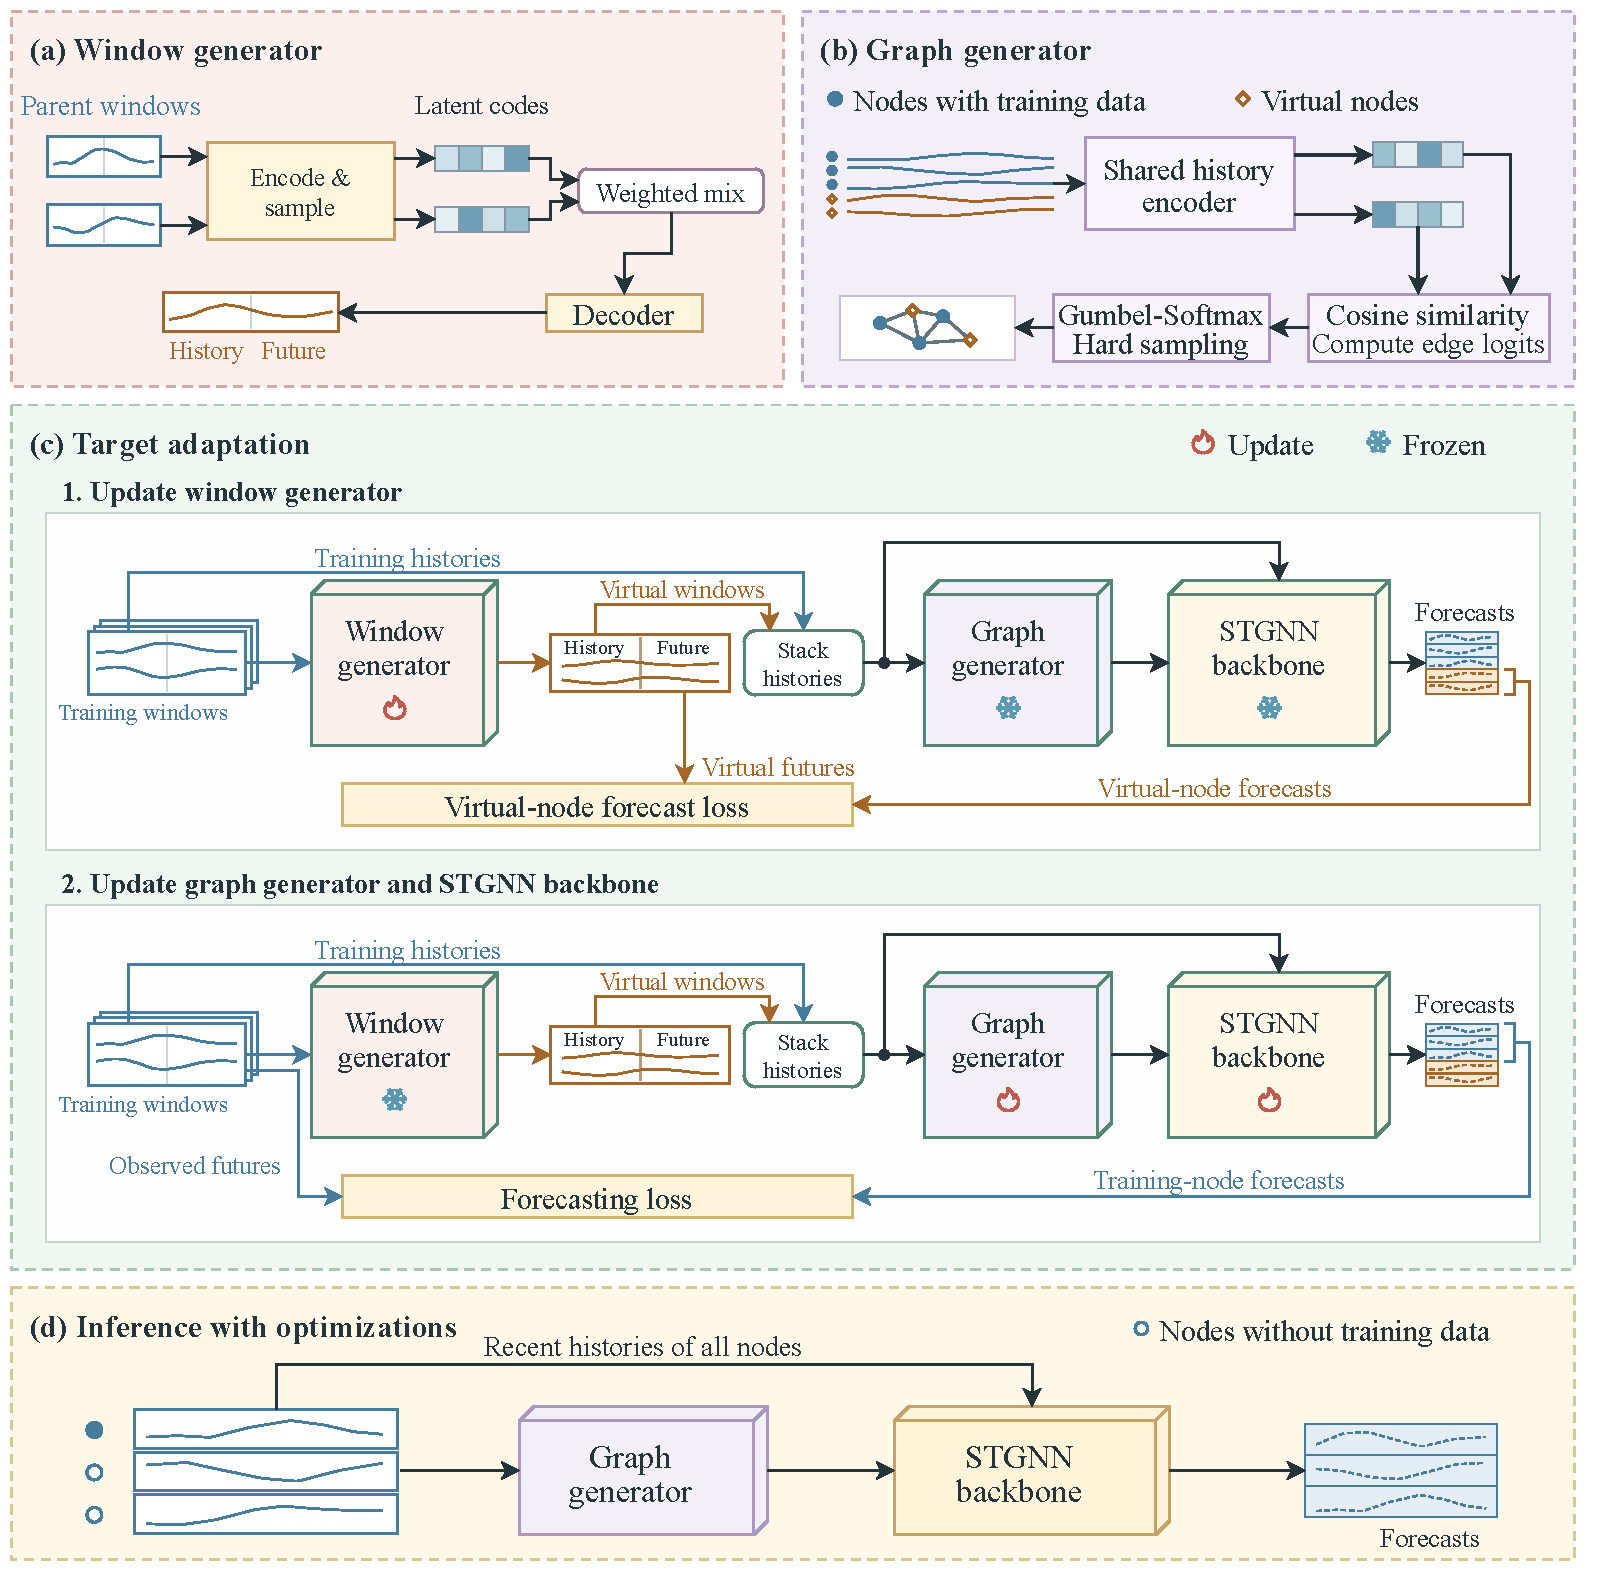
\includegraphics[width=0.92\textwidth]{images/method-overview.pdf}
\caption{CrossGEN概览。(a)面板详述窗口生成器。(b)面板详述图生成器。(c)面板展示从源端预训练权重到迁移模块的目标域适配，包括交替更新及其预测损失项。(d)面板展示禁用窗口生成器后的推理。}
\label{fig:method-overview}
\end{figure}

\subsection{窗口生成器}
\label{sec:node-generator}

\textbf{为应对捕捉超出目标训练节点观测范围的时间模式这一第一项挑战}，CrossGEN迁移在源城市观测上预训练的窗口生成器。该生成器沿用ST-FiT的增广机制，混合两个真实交通窗口的潜在编码，并将所得编码解码为虚拟训练窗口。

在目标域适配期间，真实窗口来自$\mathcal O_T$中的节点。我们使用$\mathcal S_T(x)=(x-m_T)/s_T$对目标交通观测进行标准化，其中$m_T$和$s_T>0$是由目标训练节点处训练窗口计算得到的均值和标准差；窗口生成器和STGNN骨架均输出标准化值，$\overline H_i^{(t)}$和$\overline Y_i^{(t)}$分别是$H_i^{(t)}$和$Y_i^{(t)}$的标准化版本。变分编码器~\cite{vae}将每个完整窗口$U_i^{(t)}=(\overline H_i^{(t)},\overline Y_i^{(t)})\in\mathbb R^{P+Q}$映射为高斯分布参数，随后以可调尺度采样潜在编码，
\begin{equation}
  (\mu_i^{(t)},\ell_i^{(t)})=E_\theta(U_i^{(t)}),\quad
  z_i^{(t)}=\mu_i^{(t)}+\rho\exp(\ell_i^{(t)}/2)\odot\epsilon_i^{(t)},\quad
  \epsilon_i^{(t)}\sim\mathcal N(0,I_d),
  \label{eq:latent-code}
\end{equation}
其中编码器$E_\theta$和解码器$D_\theta$在各节点间共享参数，$\rho$用于缩放采样所用的标准差，均值$\mu_i^{(t)}$、对数方差$\ell_i^{(t)}$和采样编码$z_i^{(t)}$均为$\mathbb R^d$中的向量，其中$d$为潜在维度。

随后以比例$\lambda$混合两个父窗口的编码，即$\widetilde z_k^{(t)}=\lambda z_{i_k}^{(t)}+(1-\lambda)z_{j_k}^{(t)}$，解码器将混合编码映射回完整的$P+Q$窗口$\widetilde U_k^{(t)}=D_\theta(\widetilde z_k^{(t)})$，其前$P$步构成历史$\widetilde H_k^{(t)}\in\mathbb R^P$，后$Q$步构成未来$\widetilde Y_k^{(t)}\in\mathbb R^Q$（图~\ref{fig:method-overview}(a)）。我们将虚拟历史与目标训练节点的历史拼接，用于图构建和预测（图~\ref{fig:method-overview}(c)）；在阶段1中，每个虚拟未来作为相应虚拟节点预测的监督目标。为方便起见，本节我们用$\mathcal K$索引$K$个虚拟节点，并以$\mathcal V^{+}=\mathcal O_T\cup\mathcal K$表示适配期间使用的节点集合，其中$N_{\mathcal V^{+}}=N_{\mathrm{train}}+K$个节点；矩阵$\overline H_{\mathcal V^{+}}^{(t)}\in\mathbb R^{N_{\mathcal V^{+}}\times P}$的行依次为目标训练节点的标准化历史$\overline H_i^{(t)}$和虚拟节点的生成历史$\widetilde H_k^{(t)}$。

为优化编码器和解码器，我们最小化虚拟窗口与其两个父窗口之间的平方距离以及潜在正则项。为鼓励全部$P+Q$步上的时间一致性，我们使用骨架在采样图上根据生成历史预测未来。令$\widehat{\overline Y}_{\mathcal V^{+}}^{(t)}\in\mathbb R^{N_{\mathcal V^{+}}\times Q}$为骨架对$\mathcal V^{+}$中节点的输出；对于虚拟节点$k$，我们在每个预测步$q$比较预测$\widehat{\overline Y}_{k,q}^{(t)}$与生成值$\widetilde Y_{k,q}^{(t)}$，两者均为标准化值。由此得到的窗口生成器目标为
\begin{equation}
\begin{aligned}
  \mathcal L_{\rm lat}^{(t)}&=\frac{1}{\text{$N_{\mathrm{train}}$}}\sum_{i\in\mathcal O_{T}}\sum_{r=1}^{d}
      \bigl((\mu_{i,r}^{(t)})^2+\exp(\ell_{i,r}^{(t)})-1-\ell_{i,r}^{(t)}\bigr),\\
  \mathcal L_{\rm par}^{(t)}&=\frac{1}{K(P+Q)}\sum_{k=1}^{K}
      \Bigl(\|\widetilde U_k^{(t)}-U_{i_k}^{(t)}\|_2^2+\|\widetilde U_k^{(t)}-U_{j_k}^{(t)}\|_2^2\Bigr),\\
  \mathcal L_{\rm vf}^{(t)}&=
      \text{$\displaystyle\frac{1}{KQ}\sum_{k\in\mathcal K}\sum_{q=1}^{Q}
      \left|\widehat{\overline Y}_{k,q}^{(t)}-\widetilde Y_{k,q}^{(t)}\right|$},
      \qquad\mathcal L_{\rm src}=\|\theta-\theta_S\|_2^2,\\
  \mathcal L_N^{(t)}&=\lambda_{\rm vf}\mathcal L_{\rm vf}^{(t)}+\lambda_{\rm lat}\mathcal L_{\rm lat}^{(t)}
      +\lambda_{\rm par}\mathcal L_{\rm par}^{(t)}+\lambda_{\rm src}\mathcal L_{\rm src},
\end{aligned}
  \label{eq:node-objectives}
\end{equation}
其中潜在惩罚作用于未缩放的均值和对数方差，不含~\eqref{eq:latent-code}中的采样尺度$\rho$；源惩罚$\mathcal L_{\rm src}$将$\theta$锚定到其源端取值；父窗口惩罚鼓励虚拟窗口保留两个父窗口的时间模式；而$\mathcal L_{\rm vf}^{(t)}$鼓励骨架的预测与生成的未来保持一致。

\subsection{图生成器与STGNN骨架}
\label{sec:graph-generator}

\textbf{为应对在没有预定义目标邻接矩阵的情况下推断空间依赖这一第二项挑战}，图生成器根据节点的时间历史构建它们之间的连接。适配期间，它连接目标训练节点和窗口生成器产生的虚拟节点（图~\ref{fig:method-overview}(b)）；推理时，同样的构建过程使用所有目标节点的近期历史，包括没有训练数据的节点（图~\ref{fig:method-overview}(d)）。

共享编码器首先将每个历史映射为表示，两个表示之间的余弦相似度给出边分数，
\begin{equation}
  v_a^{(t)}=g_\phi(\overline H_a^{(t)}),\quad e_a^{(t)}=\frac{v_a^{(t)}}{\max(\|v_a^{(t)}\|_2,\epsilon_e)},\quad
  s_{ab}^{(t)}=\langle e_a^{(t)},e_b^{(t)}\rangle,\quad a,b\in\mathcal V^{+} ,
  \label{eq:graph-history-scores}
\end{equation}
其中$a$和$b$遍历$\mathcal V^{+}$，$\overline H_a^{(t)}\in\mathbb R^{P}$是节点$a$的标准化历史，当$a\in\mathcal K$时$\overline H_a^{(t)}=\widetilde H_a^{(t)}$。我们将采样邻接记为$\tilde A^{(t)}=G_\phi(\overline H_{\mathcal V^{+}}^{(t)})$。为采样每条边，我们在窗口内对分数进行归一化、平移$\delta$，并以尺度$\alpha$对平移后的分数取指数，得到边存在与边不存在的对数几率；温度为$\tau$的硬Gumbel-Softmax~\cite{gumbel}采样$\operatorname{GS}^{\rm hard}_{\tau}$随后给出边，
\begin{equation}
\begin{aligned}
  r_{ab}^{(t)}&=\frac{s_{ab}^{(t)}-s_{\min}^{(t)}}{\max(s_{\max}^{(t)}-s_{\min}^{(t)},\epsilon_r)}-\delta,\\
  \ell_{ab}^{(t),\rm on}&=\exp(\alpha r_{ab}^{(t)}),\qquad
  \ell_{ab}^{(t),\rm off}=\exp(-\alpha r_{ab}^{(t)}),\\
  \tilde A_{ab}^{(t)}&=\left[\operatorname{GS}^{\rm hard}_{\tau}(\ell_{ab}^{(t),\rm on},\ell_{ab}^{(t),\rm off})\right]_{\rm on},
  \qquad \tau>0 ,
\end{aligned}
  \label{eq:sparse-graph}
\end{equation}
因此图是离散的，同时梯度仍然通过采样的边传播。这里$s_{\min}^{(t)}$和$s_{\max}^{(t)}$是窗口内的最小和最大分数，$\epsilon_e$和$\epsilon_r$是数值稳定性常数，所得邻接矩阵$\tilde A^{(t)}$的形状为$N_{\mathcal V^{+}}\times N_{\mathcal V^{+}}$。共享编码器和评分函数适用于不同规模的节点集合，分数越高，边越容易被纳入采样图。CrossGEN迁移图生成器的学习参数，并从目标城市可用的历史中采样新的边。

STGNN骨架$F_\psi$以标准化节点历史$\overline H^{(t)}$和图生成器产生的邻接矩阵$\tilde A^{(t)}$为输入，为每个节点输出$Q$步预测；结合第~\ref{sec:target-adaptation}~节的残差校正，它还接收关系矩阵$C^{(t)}$，因此$\widehat{\overline Y}^{(t)}=F_\psi(\overline H^{(t)},\tilde A^{(t)},C^{(t)})$。适配期间，骨架接收$\overline H_{\mathcal V^{+}}^{(t)}$（图~\ref{fig:method-overview}(c)）；推理时，它接收所有目标节点的标准化近期历史$\overline H_{\mathcal V_T}^{(t)}$（图~\ref{fig:method-overview}(d)）。其模块遵循STGCN设计~\cite{stgcn}，且$\psi$由所有节点共享，因此骨架同样适用于真实节点和虚拟节点。

\subsection{目标域适配与推理}
\label{sec:target-adaptation}
\label{sec:optimization-inference}

\textbf{为应对源目标不匹配这一第三项挑战}，我们采用\emph{目标域适配}流程，在适配迁移模块的同时限制其参数偏离预训练值。CrossGEN使用源端预训练权重初始化窗口生成器、图生成器和骨架。CrossGEN-W仅使用源端预训练权重初始化窗口生成器，并从零初始化另外两个模块。NT从零初始化全部三个模块。这些配置因此在不同模块是否接收源初始化上有所区别。三者都根据目标训练节点和虚拟节点的历史构建目标端边（图~\ref{fig:method-overview}(c)）。迁移要求$P$和$Q$匹配且参数形状兼容，但不要求两个节点集合之间存在对应关系。

目标端初始化的门控残差校正将骨架的图卷积消息适配到目标城市。为限制参数偏离，我们将源端加载的参数正则化到其预训练值附近，并在初始轮次冻结它们。具体地，校正将$\overline H_{\mathcal V^{+}}^{(t)}$的第$i$行中心化并归一化为$u_i^{(t)}$，并通过$u_i^{(t)}$与$W_\phi u_i^{(t)}$的平均余弦相似度对每对节点评分，
\begin{equation}
  b_{ij}^{(t)}=\left[\tfrac12\left((u_i^{(t)})^\top u_j^{(t)}+(W_\phi u_i^{(t)})^\top(W_\phi u_j^{(t)})\right)\right]_{[0,1]},
  \qquad b_{ii}^{(t)}=0 ,
  \label{eq:correction-scores}
\end{equation}
其中$[\cdot]_{[0,1]}$截断到单位区间。令$\Pi^{(t)}\in[0,1]^{N_{\mathcal V^{+}}\times N_{\mathrm{train}}}$编码时间$t$窗口的父节点。对于$i\in\mathcal O_T$，我们设$\Pi_{i,i}^{(t)}=1$。对于父节点为$i_k$和$j_k$的虚拟节点$k$，我们设$\Pi_{k,i_k}^{(t)}=\lambda$，$\Pi_{k,j_k}^{(t)}=1-\lambda$。稀疏关系矩阵$C^{(t)}\in\mathbb R^{N_{\mathcal V^{+}}\times N_{\mathcal V^{+}}}$每行最多保留四个最大元素，并按保留和归一化每一行；虚拟节点的行随后按其父权重$\Pi^{(t)}$混合。门控残差消息随后被加到图卷积上，
\begin{equation}
\begin{aligned}
  Z^{(t,l)}&=\operatorname{TempConv}_1(H^{(t,l)}),\\
  H^{(t,l+1)}&=\operatorname{ChebConv}(Z^{(t,l)};\tilde A^{(t)})+\tanh(\gamma)\,R(C^{(t)}Z^{(t,l)}-Z^{(t,l)}),
\end{aligned}
  \label{eq:sparse-correction}
\end{equation}
其中$H^{(t,l)}$是时间$t$窗口第$l$个模块的输入（上标$(t,l)$分别索引窗口时间和网络模块），$R$为逐模块无偏置映射，$\gamma$为门控。对于$\mathcal V^{+}$中的$N_{\mathcal V^{+}}$个节点，$Z^{(t,l)}\in\mathbb R^{L_l\times N_{\mathcal V^{+}}\times d_l}$，其中$L_l$和$d_l$是第一次时间卷积后的时间步数和特征通道数。在每个时间步，$C^{(t)}$沿$Z^{(t,l)}$的节点轴作用，$R$沿残差的特征轴作用。门控从零开始，因此残差项初始为零。校正参数属于$\psi$，但不参与源加载和源正则化。图~\ref{fig:method-overview}(c)和(d)中的STGNN骨架包含此校正。

\paragraph{交替目标域适配。}
适配期间各模块相互依赖。窗口生成器使用骨架的预测评价其虚拟窗口。图生成器从拼接的真实和虚拟历史中采样图，STGNN骨架使用这些历史和采样图进行预测。我们使用窗口生成器目标和下面的预测目标，交替进行图~\ref{fig:method-overview}(c)所示的两个阶段来训练各模块。

在阶段1中，我们以$\mathcal L_N^{(t)}$更新窗口生成器，并冻结图生成器和STGNN骨架。虚拟节点预测损失比较虚拟节点的预测未来与其生成未来。在阶段2中，我们冻结窗口生成器，联合更新图生成器和STGNN骨架。预测损失比较训练节点预测与观测未来。正则项将源端加载的参数锚定到其预训练值，
\begin{equation}
\begin{aligned}
  C^{(t)}&=C_\phi(\overline H_{\mathcal V^{+}}^{(t)},\Pi^{(t)}),\qquad
  \widehat{\overline Y}_{\mathcal V^{+}}^{(t)}=F_\psi(\overline H_{\mathcal V^{+}}^{(t)},\tilde A^{(t)},C^{(t)}),\\
  \widehat Y_{\mathcal O_{T}}^{(t)}&=\mathcal S_T^{-1}([\widehat{\overline Y}_{\mathcal V^{+}}^{(t)}]_{\mathcal O_{T}}),\\
  \mathcal L_{\rm pred}^{(t)}&=\frac{1}{\text{$N_{\mathrm{train}}$}Q}\sum_{i\in\mathcal O_{T}}\sum_{q=1}^{Q}
      |\widehat Y_{i,q}^{(t)}-Y_{i,q}^{(t)}|,\\
  \mathcal L_{GF}^{(t)}&=\mathcal L_{\rm pred}^{(t)}
      +\lambda_{GF}\sum_{p\in\mathcal P_S}\|p-p_S\|_2^2,
\end{aligned}
  \label{eq:target-objectives}
\end{equation}
其中$\mathcal P_S$汇集两个模块的源端加载参数。记号$[\cdot]_{\mathcal O_T}$选择目标训练节点的行。图~\ref{fig:method-overview}(c)中的两个损失框分别展示预测项$\mathcal L_{\rm vf}^{(t)}$和$\mathcal L_{\rm pred}^{(t)}$。这样，窗口生成器为预测提供虚拟窗口，而图生成器为骨架提供图。

\paragraph{全节点推理。}
推理时（图~\ref{fig:method-overview}(d)），我们禁用窗口生成器，并将所有目标节点的近期历史标准化为$\overline H_{\mathcal V_T}^{(t)}=\mathcal S_T(H_{\mathcal V_T}^{(t)})$。适配后的图生成器$G_{\phi^\star}$根据这些历史构建图$\tilde A^{(t)}$。STGNN骨架$F_{\psi^\star}$使用相同的历史、生成的图和由$C_{\phi^\star}$计算的残差关系$C^{(t)}$预测所有目标节点。我们在计算评价指标之前，对标准化预测$\widehat{\overline Y}_{\mathcal V_T}^{(t)}$应用$\mathcal S_T^{-1}$，得到$\widehat Y_{\mathcal V_T}^{(t)}$。


\subsection{源数据集选择}
\label{sec:source-selection}

为对候选源数据集排序，我们根据训练划分中选定源节点和目标训练节点的历史交通观测计算统计量。这些统计量不使用目标测试观测，也不要求源节点与目标节点对应。我们为候选源数据集$S$和目标数据集$T$定义节点距离$A(S,T)$和关系距离$D(S,T)$。

节点距离$A(S,T)$比较每个节点的七项统计量，包括相邻时间步之间的归一化平均绝对变化和六个滞后的自相关。关系距离$D(S,T)$比较节点对之间残差相关性的分布。我们在控制预测节点的近期观测以及日周期和周周期后，在各数据集内计算这些相关性。

分数为
\[
s_{\text{CrossGEN-W}}(S,T)=A(S,T),\qquad
s_{\text{CrossGEN}}(S,T)=0.25A(S,T)+0.75D(S,T).
\]
我们按分数从低到高对候选源排序。分数权重是使用早期迁移结果校准的，因此第~\ref{sec:source}~节中的源排序分析是回顾性的。这些分数提供排序规则，而非正迁移的保证。

\section{实验}\label{sec:results}
\begin{samepage}
我们的实验回答以下四个研究问题。
\begingroup
\DeclareRobustCommand{\revisedresearchquestions}{%
  \begin{itemize}
  \item \textbf{RQ1.} 与各基线相比，CrossGEN在目标节点，尤其是没有训练数据的节点上的交通预测效果如何？
  \item \textbf{RQ2.} CrossGEN中哪些模块使用源端预训练权重初始化，如何影响目标训练数据上的预测？
  \item \textbf{RQ3.} 对于给定目标数据集，源数据集的选择如何影响预测性能？
  \item \textbf{RQ4.} 目标训练节点覆盖如何影响CrossGEN的预测性能？
  \end{itemize}%
}
\revisedresearchquestions
\endgroup
\end{samepage}

\subsection{实验设置}
\label{sec:experimental-settings}


\noindent\textbf{数据集。}我们使用七个数据集（表~\ref{tab:datasets}），包括五个交通流量数据集和两个交通指数数据集。

\DeclareRobustCommand{\datasetvariablelist}{%
  \begin{itemize}
  \item \emph{交通流量数据集。}交通流量是每个间隔内传感器计数的车辆数。\textbf{PEMS03}、\textbf{PEMS04}和\textbf{PEMS08}是基于加州交通绩效测量系统（PeMS）~\cite{pems}数据的现有基准，传感器分别位于第3、第4和第8区~\cite{stfit}。\textbf{CA03}和\textbf{CA06}是我们从LargeST的加利福尼亚数据集~\cite{largest}中分别选择第3和第6区传感器构建的子集。
  \item \emph{交通指数数据集。}交通指数是衡量道路级交通拥堵的指标。\textbf{Shenzhen}和\textbf{Chengdu}是现有的交通指数数据集，观测分别来自深圳市中心和成都核心城区的道路。两个数据集均来自滴滴出行GAIA计划~\cite{stgfsl}，并通过OpenCity~\cite{opencity}分发。
  \end{itemize}%
}
\datasetvariablelist

\begin{table}[!ht]
\centering
\DeclareRobustCommand{\datasetstatisticstable}{%
\caption{数据集特征。}
\label{tab:datasets}
\footnotesize
\setlength{\tabcolsep}{1pt}
\renewcommand{\arraystretch}{1.1}
\begin{tabular*}{\linewidth}{@{\extracolsep{\fill}}lllrr@{}}
\hline
数据集 & 地点 & 变量 & 节点数 & 时间步数 \\
\hline
PEMS03 & 美国加州交通局第3区 & 交通流量 & 358 & 26,208 \\
PEMS04 & 美国加州交通局第4区 & 交通流量 & 307 & 16,992 \\
PEMS08 & 美国加州交通局第8区 & 交通流量 & 170 & 17,856 \\
CA03 & 美国加州交通局第3区 & 交通流量 & 441 & 25,920 \\
CA06 & 美国加州交通局第6区 & 交通流量 & 456 & 25,920 \\
Shenzhen & 中国深圳 & 交通指数 & 627 & 17,280 \\
Chengdu & 中国成都 & 交通指数 & 524 & 17,280 \\
\hline
\end{tabular*}%
}
\datasetstatisticstable
\end{table}

\begingroup
\DeclareRobustCommand{\baselinecomparison}{%
  \noindent\textbf{基线。}我们考虑以下基线。
  \begin{itemize}
  \item \textbf{历史平均（HA）}~\cite{dai2020hstgcn}对历史交通观测取平均。
  \item \textbf{FC-LSTM}~\cite{sutskever2014seq2seq}使用全连接LSTM预测交通。
  \item \textbf{STGCN}~\cite{stgcn}结合图卷积和时间卷积。
  \item \textbf{STGODE}~\cite{fang2021stgode}结合图常微分方程与时间卷积。
  \item \textbf{ST-FiT}~\cite{stfit}使用虚拟节点和学习图。
  \end{itemize}%
}
\begin{samepage}
\baselinecomparison
\end{samepage}
\endgroup

\begingroup
\DeclareRobustCommand{\evaluationmetrics}{%
\begin{samepage}
  \textbf{评价指标。}令$\mathcal T_{\mathrm{test}}$包含进行测试预测所对应的时间索引$t$，其中$T_{\mathrm{test}}=|\mathcal T_{\mathrm{test}}|$。对于包含$N_{\mathcal A}$个目标节点的集合$\mathcal A\subseteq\mathcal V_T$，预测步$q$处的平均绝对误差（MAE）为
\[
  \operatorname{MAE}_{q}(\mathcal A)
  = \frac{1}{T_{\mathrm{test}}N_{\mathcal A}}
    \sum_{t\in\mathcal T_{\mathrm{test}}}\sum_{i\in\mathcal A}
    \left|\widehat Y_{i,q}^{(t)}-Y_{i,q}^{(t)}\right|.
\]
我们在原始数据尺度上计算MAE，并对全部$Q$个预测步取平均。
\end{samepage}
我们报告$\mathcal A\in\{\mathcal V_T,\mathcal O_T,\mathcal U_T\}$上的MAE。
采用五个随机种子训练时，我们报告五次运行的MAE均值。我们对全部目标节点上的MAE实施双侧配对$t$检验，按随机种子匹配运行，以比较CrossGEN与其他方法。我们使用未经校正的$p$值。
}
\noindent\evaluationmetrics
\endgroup

\noindent\textbf{实现设置。}
历史长度和预测长度均为12个时间步（$P=Q=12$）。对于间隔为5min的交通流量，预测时域为1h；对于间隔为10min的交通指数，预测时域为2h。

主要实验使用$N_{\mathrm{train}}=\lfloor 0.1 N_T\rfloor$个目标训练节点。
在我们的运行中，我们采用按时间顺序的6:2:2划分来划分训练集、验证集和测试集。





每个主要实验使用指定的源数据集和目标数据集。我们使用五个随机种子训练和评价CrossGEN，并在每个目标数据集上使用相同种子运行ST-FiT。
我们在所有具有历史交通观测的源节点上预训练50轮。
我们在目标数据上训练最多100轮，并在连续20次验证检查无改善后提前停止。
训练使用Adam（学习率$2\times10^{-3}$，权重衰减$10^{-4}$），批大小为4。
窗口生成器使用$d=64$，$\lambda=0.5$，$K=N_{\mathrm{train}}$。图生成器使用$\delta=0.9$，$\alpha=10$，$\tau=1$。





CrossGEN在所列的各个源数据集上预训练，并使用相同的目标训练节点和时间划分进行适配。所有其他方法仅使用目标训练数据：ST-FiT在该数据上从头训练，四种参考方法在目标测试数据上评价。我们报告CA03、CA06、Shenzhen和Chengdu上的MAE；对于PEMS03、PEMS04和PEMS08，则使用Lei等人~\cite{stfit}表~1中的参考值。所有方法均在相同的目标测试数据和全部目标节点上评价。

\subsection{总体结果（RQ1）}
\label{sec:overall-results}









表~\ref{tab:main-results}报告交通流量和交通指数实验中全部目标节点上的结果。仅使用目标训练数据的方法在每个目标数据集上各有一个结果，而表中唯一的跨城市方法CrossGEN每行对应一个结果。

在全部交通指数实验以及除CA06到PEMS08以外的全部交通流量实验中，CrossGEN的MAE低于所有其他方法。在PEMS08上，以CA06为源时ST-FiT的MAE最低，而以PEMS03或PEMS04为源时CrossGEN的MAE低于ST-FiT。源预训练可以帮助窗口生成器捕捉目标训练数据中未被充分表示的时间模式，并帮助图生成器从目标历史中识别有用的邻居。这些收益取决于所学时间模式和空间依赖能否适用于目标域。CA06到PEMS08的结果与空间依赖不匹配的解释一致。当迁移的图生成器和STGNN骨架偏向于不同于目标域的空间依赖时，朝向源权重的正则化可能使模型更难仅利用一部分目标节点的数据调整边分数和邻居聚合。

\begin{table}[t]
\centering
\caption{全部目标节点上的预测结果。}
\label{tab:main-results}
\footnotesize
\setlength{\tabcolsep}{2.2pt}
\begin{tabular}{@{}llrrrr@{\hspace{9pt}}rr@{}}
\hline
\shortstack[l]{目标\\数据集} & \shortstack[l]{源\\数据集} &
HA & FC-LSTM & STGCN & STGODE & ST-FiT & CrossGEN \\
\hline
\multirow{3}{*}{PEMS03} & CA06 &
  \multirow{3}{*}{32.47} & \multirow{3}{*}{20.56} &
  \multirow{3}{*}{23.22} & \multirow{3}{*}{31.05} &
  \multirow{3}{*}{18.86} & \textbf{18.35} \\
 & PEMS04 & & & & & & \textbf{18.03} \\
 & PEMS08 & & & & & & \textbf{18.43} \\[3pt]
\multirow{3}{*}{PEMS04} & CA06 &
  \multirow{3}{*}{41.98} & \multirow{3}{*}{28.17} &
  \multirow{3}{*}{32.60} & \multirow{3}{*}{34.35} &
  \multirow{3}{*}{25.23} & \textbf{24.57} \\
 & PEMS03 & & & & & & \textbf{24.83} \\
 & PEMS08 & & & & & & \textbf{24.55} \\[3pt]
\multirow{3}{*}{PEMS08} & CA06 &
  \multirow{3}{*}{34.56} & \multirow{3}{*}{30.52} &
  \multirow{3}{*}{41.67} & \multirow{3}{*}{30.00} &
  \multirow{3}{*}{23.15} & 23.55 \\
 & PEMS03 & & & & & & \textbf{23.00} \\
 & PEMS04 & & & & & & 23.05 \\[3pt]
\multirow{2}{*}{CA03} & CA06 &
  \multirow{2}{*}{36.65} & \multirow{2}{*}{26.43} &
  \multirow{2}{*}{32.64} & \multirow{2}{*}{30.98} &
  \multirow{2}{*}{21.35} & \textbf{21.15} \\
 & PEMS04 & & & & & & \textbf{21.34} \\[3pt]
\multirow{3}{*}{CA06} & CA03 &
  \multirow{3}{*}{30.28} & \multirow{3}{*}{28.23} &
  \multirow{3}{*}{21.74} & \multirow{3}{*}{24.74} &
  \multirow{3}{*}{16.74} & \textbf{16.07} \\
 & PEMS03 & & & & & & \textbf{16.36} \\
 & PEMS04 & & & & & & \textbf{16.49} \\
\hline
Shenzhen & Chengdu & 4.27 & 3.68 & 3.17 & 3.37 & 2.90 & \textbf{2.77} \\
Chengdu & Shenzhen & 5.02 & 4.40 & 3.63 & 4.14 & 3.12 & \textbf{3.07} \\
\hline
\end{tabular}\par
\end{table}

\subsection{消融研究（RQ2）}
\label{sec:configuration-scope}

\begingroup
\DeclareRobustCommand{\ablationpar}{\par}



\DeclareRobustCommand{\ablationvariants}{%
  \begin{samepage}
    每个模型变体在目标训练数据上训练全部三个模块。
    \begin{enumerate}
    \item \textbf{NT（无迁移）}从零初始化每个模块。
    \item \textbf{CrossGEN-W}（W表示窗口）仅使用源端预训练权重初始化窗口生成器，并从零初始化图生成器和STGNN骨架。
    \item \textbf{CrossGEN}使用源端预训练权重初始化窗口生成器、图生成器和STGNN骨架。
    \end{enumerate}
  \end{samepage}%
}
\ablationvariants
CrossGEN-W有助于分两个阶段评估迁移。比较NT与CrossGEN-W衡量使用源端预训练权重初始化窗口生成器的效果。比较CrossGEN-W与CrossGEN评价迁移图生成器和STGNN骨架并应用相应目标域适配设计的联合效果。
\ablationpar
表~\ref{tab:group-results}分别报告有训练数据和没有训练数据的目标节点的结果。
与NT相比，CrossGEN-W和CrossGEN分别在14个交通流量实验中的10个和11个实验以及两个交通指数实验中降低了全部目标节点上的MAE。该比较证实了迁移的有效性：使用源端预训练权重初始化窗口生成器能改善预测，额外迁移图生成器和骨架还会带来进一步提升。然而，在PEMS08上，CrossGEN-W在所有实验中均优于CrossGEN。
\par
\endgroup

\begin{table}[!htbp]
\centering
\caption{按目标节点组的消融结果。}
\label{tab:group-results}
\footnotesize
\setlength{\tabcolsep}{3pt}
\begin{tabular}{@{}llrr|rr|rr@{}}
\hline
\multirow{2}{*}{\shortstack[l]{目标\\数据集}} &
\multirow{2}{*}{\shortstack[l]{源\\数据集}} &
\multicolumn{2}{c|}{NT} & \multicolumn{2}{c|}{CrossGEN-W} & \multicolumn{2}{c}{CrossGEN} \\
 & & $\mathcal O_{T}$ & $\mathcal U_T$ & $\mathcal O_{T}$ & $\mathcal U_T$ & $\mathcal O_{T}$ & $\mathcal U_T$ \\
\hline
PEMS03 & CA06 & 18.35 & 18.92 & \textbf{18.06} & 18.37 & 18.21 & \textbf{18.37} \\
PEMS03 & PEMS04 & 18.35 & 18.92 & 18.42 & 18.34 & \textbf{17.90} & \textbf{18.04} \\
PEMS03 & PEMS08 & 18.35 & 18.92 & 18.97 & 18.59 & \textbf{17.71} & \textbf{18.51} \\
PEMS04 & CA06 & 23.80 & 25.39 & 24.17 & 25.82 & \textbf{23.26} & \textbf{24.71} \\
PEMS04 & PEMS03 & 23.80 & 25.39 & \textbf{22.59} & 25.28 & 23.60 & \textbf{24.96} \\
PEMS04 & PEMS08 & 23.80 & 25.39 & \textbf{23.24} & 25.31 & 23.92 & \textbf{24.62} \\
PEMS08 & CA06 & 24.79 & 22.97 & \textbf{23.98} & \textbf{22.21} & 25.11 & 23.38 \\
PEMS08 & PEMS03 & 24.79 & 22.97 & \textbf{23.13} & \textbf{22.03} & 24.71 & 22.81 \\
PEMS08 & PEMS04 & 24.79 & 22.97 & \textbf{23.01} & \textbf{21.36} & 24.47 & 22.89 \\
CA03 & CA06 & 19.25 & 21.58 & 19.49 & 21.64 & \textbf{18.99} & \textbf{21.39} \\
CA03 & PEMS04 & 19.25 & \textbf{21.58} & 19.72 & 21.95 & \textbf{18.45} & 21.66 \\
CA06 & CA03 & 18.29 & 16.57 & 17.65 & 16.28 & \textbf{17.31} & \textbf{15.93} \\
CA06 & PEMS03 & 18.29 & 16.57 & \textbf{17.31} & 16.23 & 18.42 & \textbf{16.13} \\
CA06 & PEMS04 & 18.29 & 16.57 & 17.61 & \textbf{16.30} & \textbf{17.46} & 16.39 \\
\hline
Shenzhen & Chengdu & 2.82 & 2.91 & 2.68 & 2.83 & \textbf{2.68} & \textbf{2.78} \\
Chengdu & Shenzhen & 2.83 & 3.16 & 2.87 & 3.16 & \textbf{2.76} & \textbf{3.10} \\
\hline
\end{tabular}\par
\end{table}

\subsection{源数据集选择（RQ3）}
\label{sec:source}
源预训练期间学到的时间模式和空间依赖取决于源数据集，因此源数据集的选择可能影响目标MAE。图~\ref{fig:source-ranking-bars}按MAE对CrossGEN下每个交通流量目标的候选源进行排序。每个交通指数目标只有一个候选源，因此该分析聚焦于交通流量目标。

\begin{figure}[!htbp]
\centering
\begin{subfigure}[t]{0.49\linewidth}
\centering
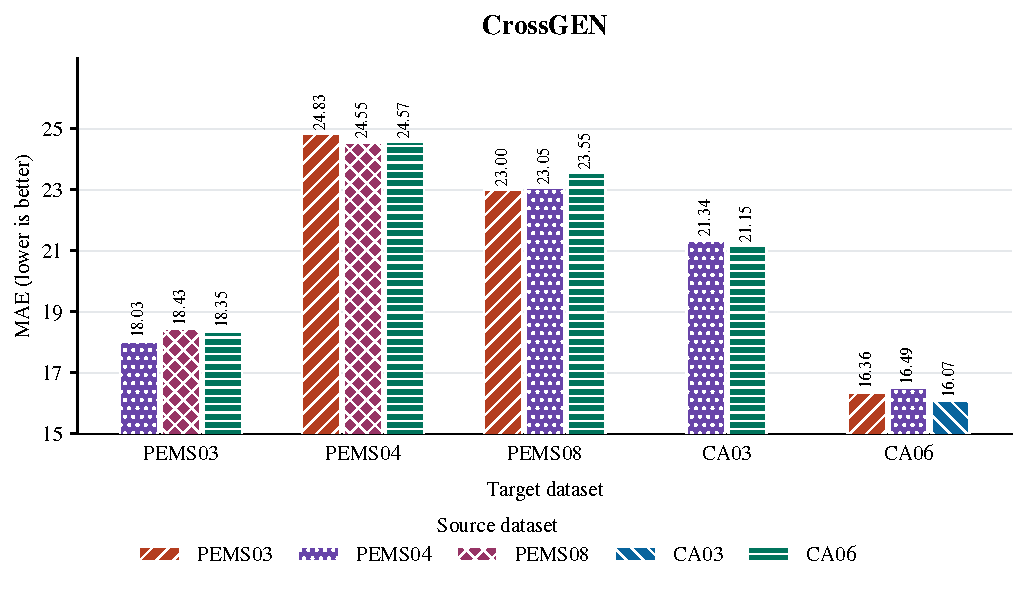
\includegraphics[width=\linewidth]{image/source-ranking-bars-crossgen.pdf}
\caption{CrossGEN的源数据集排名。每组柱状条显示某个交通流量目标下各候选源的MAE；越低越好。}
\label{fig:source-ranking-bars}
\end{subfigure}\hfill
\begin{subfigure}[t]{0.49\linewidth}
\centering
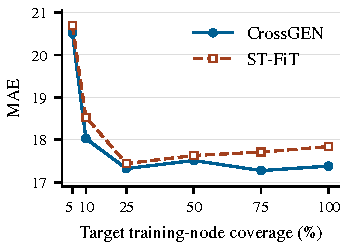
\includegraphics[width=\linewidth]{image/training-node-coverage.pdf}
\caption{PEMS03上按目标训练节点覆盖的MAE。ST-FiT的数值取自Lei等人~\cite{stfit}的图~3(a)。}
\label{fig:training-node-coverage}
\end{subfigure}
\caption{源数据集选择与目标训练节点覆盖。}
\end{figure}

首选源随目标而变化。例如，在PEMS03上，最低MAE来自PEMS04；在PEMS08上，则来自PEMS03，说明最佳源取决于目标数据集。

为考察更相似的数据集是否产生更低的MAE，我们将这些观测排名与第~\ref{sec:source-selection}~节定义的相异度分数产生的排名进行比较。

对于每个目标数据集，我们两两比较候选源。在13个比较中的9个中，分数较低的源取得较低的MAE；在5个交通流量目标中的4个中，分数最低的源取得最低MAE。在PEMS08上，PEMS03在两项度量下均排名第一，而分数将CA06排在PEMS04之前，尽管PEMS04的MAE更低。

分数与MAE之间的一致性源于两个距离所衡量的内容。节点距离$A(S,T)$衡量两个城市时间模式的相似程度，表明源端预训练的窗口生成器能为目标贡献多少；关系距离$D(S,T)$衡量两地空间依赖的相似程度，表明迁移的图生成器和骨架能多好地适配。CrossGEN同时迁移这两类模块，其分数以较大权重（0.75）组合关系距离。这种回顾性一致表明，这些统计量有助于为给定目标筛选源，但将其用作选择规则仍需在分数校准之外的实验上进行验证。

\subsection{目标训练节点覆盖的影响（RQ4）}
\label{sec:training-node-coverage}



主要实验使用约10\%的目标训练节点覆盖。为考察预测对目标训练数据量的敏感程度，我们改变PEMS03中提供用于训练的历史交通观测的节点比例。图~\ref{fig:training-node-coverage}展示在所评价覆盖水平下CrossGEN的MAE，以及已发表的ST-FiT曲线。推理时所有目标节点仍提供近期观测。

两条曲线均在最低覆盖水平之间呈现最大的MAE下降。MAE在中间覆盖水平继续下降，并在较高覆盖水平于较窄范围内波动。

在低覆盖水平，增加训练节点会提供来自更多位置的历史和预测目标。这可以帮助CrossGEN将窗口生成器适配到目标时间模式，并在更广泛的目标观测范围上训练图生成器和STGNN骨架。在较高覆盖水平，额外节点对训练数据中已表示的模式可能贡献较少信息。

在PEMS03上，主要实验所用的覆盖水平处于MAE对提供训练数据的节点数量最敏感的范围。

\section{结论}\label{sec:discussion}

本文提出用于有限目标训练节点覆盖下跨城市交通预测的CrossGEN。
CrossGEN从源城市迁移窗口生成器、图生成器和STGNN骨架的预训练权重，并使用目标训练数据适配这些模块。
我们的实验表明，当只有少量目标节点提供训练数据时，跨城市迁移可以改善其余节点的预测。



\label{sec:conclusion}

% 匿名投稿：致谢已注释；定稿版本恢复。
% \begin{credits}
% \subsubsection{\ackname}
% OpenAI Codex在作者提供的方法、推导和记录基础上，协助了稿件组织、起草、修订、翻译和文献总结；实验表准备（第~\ref{sec:results}~节）；排序/误差检查（第~\ref{sec:source}~节）；以及可编辑方法图（图~\ref{fig:method-overview}）的设计、绘制和导出。
%
% \end{credits}

% LNCS参考文献样式；键与书目元数据保留。
\begin{thebibliography}{30}
\bibitem{boukerche2020traffic} Boukerche, A., Wang, J.: Machine Learning-based traffic prediction models for Intelligent Transportation Systems. Comput. Netw. \textbf{181}, 107530 (2020).
\bibitem{yin2022traffic} Yin, X., Wu, G., Wei, J., Shen, Y., Qi, H., Yin, B.: Deep Learning on Traffic Prediction: Methods, Analysis, and Future Directions. IEEE Trans. Intell. Transp. Syst. \textbf{23}(6), 4927--4943 (2022).
\bibitem{yuan2021traffic} Yuan, H., Li, G.: A Survey of Traffic Prediction: from Spatio-Temporal Data to Intelligent Transportation. Data Sci. Eng. \textbf{6}(1), 63--85 (2021). % https://doi.org/10.1007/s41019-020-00151-z
\bibitem{stfit} Lei, Z., Dong, Y., Li, J., Chen, C.: ST-FiT: Inductive Spatial-Temporal Forecasting with Limited Training Data. In: Proc. AAAI, pp. 12031--12039 (2025).
\bibitem{stgfsl} Lu, B., Gan, X., Zhang, W., Yao, H., Fu, L., Wang, X.: Spatio-Temporal Graph Few-Shot Learning with Cross-City Knowledge Transfer. In: Proc. ACM SIGKDD, pp. 1162--1172 (2022). 
\bibitem{transgtr} Jin, Y., Chen, K., Yang, Q.: Transferable Graph Structure Learning for Graph-Based Traffic Forecasting Across Cities. In: Proc. ACM SIGKDD, pp. 1032--1043 (2023).
\bibitem{stsurvey} Jin, G., Liang, Y., Fang, Y., Shao, Z., Huang, J., Zhang, J., Zheng, Y.: Spatio-Temporal Graph Neural Networks for Predictive Learning in Urban Computing: A Survey. IEEE Trans. Knowl. Data Eng. \textbf{36}(10), 5388--5408 (2024). 
\bibitem{stgcn} Yu, B., Yin, H., Zhu, Z.: Spatio-Temporal Graph Convolutional Networks: A Deep Learning Framework for Traffic Forecasting. In: Proc. IJCAI, pp. 3634--3640 (2018). 
\bibitem{dcrnn} Li, Y., Yu, R., Shahabi, C., Liu, Y.: Diffusion Convolutional Recurrent Neural Network: Data-Driven Traffic Forecasting. In: Proc. ICLR (2018).
\bibitem{graphwavenet} Wu, Z., Pan, S., Long, G., Jiang, J., Zhang, C.: Graph WaveNet for Deep Spatial-Temporal Graph Modeling. In: Proc. IJCAI, pp. 1907--1913 (2019). 
\bibitem{agcrn} Bai, L., Yao, L., Li, C., Wang, X., Wang, C.: Adaptive Graph Convolutional Recurrent Network for Traffic Forecasting. In: Advances in Neural Information Processing Systems, vol. 33, pp. 17804--17815 (2020).
\bibitem{mtgnn} Wu, Z., Pan, S., Long, G., Jiang, J., Chang, X., Zhang, C.: Connecting the Dots: Multivariate Time Series Forecasting with Graph Neural Networks. In: Proc. ACM SIGKDD, pp. 753--763 (2020). 
\bibitem{ignnk} Wu, Y., Zhuang, D., Labbe, A., Sun, L.: Inductive Graph Neural Networks for Spatiotemporal Kriging. In: Proc. AAAI, pp. 4478--4485 (2021). 
\bibitem{increase} Zheng, C., Fan, X., Wang, C., Qi, J., Chen, C., Chen, L.: INCREASE: Inductive Graph Representation Learning for Spatio-Temporal Kriging. In: Proc. ACM Web Conf., pp. 673--683 (2023). 
\bibitem{frigate} Gupta, M., Kodamana, H., Ranu, S.: Frigate: Frugal Spatio-temporal Forecasting on Road Networks. In: Proc. ACM SIGKDD, pp. 649--660 (2023). 
\bibitem{vae} Kingma, D.P., Welling, M.: Auto-Encoding Variational Bayes. In: Proc. ICLR (2014).
\bibitem{metast} Yao, H., Liu, Y., Wei, Y., Tang, X., Li, Z.: Learning from Multiple Cities: A Meta-Learning Approach for Spatial-Temporal Prediction. In: Proc. World Wide Web Conf., pp. 2181--2191 (2019). 
\bibitem{mtpb} Liu, Z., Zheng, G., Yu, Y.: Multi-scale Traffic Pattern Bank for Cross-city Few-shot Traffic Forecasting. ACM Trans. Knowl. Discov. Data \textbf{19}(4), Art. no. 94 (2025). 
\bibitem{stan} Fang, Z., Wu, D., Pan, L., Chen, L., Gao, Y.: When Transfer Learning Meets Cross-City Urban Flow Prediction: Spatio-Temporal Adaptation Matters. In: Proc. IJCAI, pp. 2030--2036 (2022). 
\bibitem{sert} Liu, Z., Sun, Z., Zhang, J., Zhang, B., Tong, P.: Regional Knowledge Transfer for Urban Traffic Flow Prediction via Satellite Imagery Assisted Contrastive Domain Adaptation. IEEE Trans. Intell. Transp. Syst. \textbf{26}(11), 19120--19134 (2025). 
\bibitem{traffictl} Huang, Y., Song, X., Zhu, Y., Zhang, S., Yu, J.J.Q.: Traffic Prediction With Transfer Learning: A Mutual Information-Based Approach. IEEE Trans. Intell. Transp. Syst. \textbf{24}(8), 8236--8252 (2023). 
\bibitem{crosscity} Deng, Z., Wu, Z., Su, L., Zhang, X., Wang, Y., Huang, Q.: Cross-City Correlation Learning for Traffic Forecasting. IEEE Trans. Intell. Transp. Syst. \textbf{27}(2), 2252--2267 (2026). 
\bibitem{gumbel} Jang, E., Gu, S., Poole, B.: Categorical Reparameterization with Gumbel-Softmax. In: Proc. ICLR (2017).
\bibitem{pems} California Department of Transportation: Caltrans Performance Measurement System (PeMS). https://pems.dot.ca.gov/, last accessed 2026/11/16.
\bibitem{largest} Liu, X., Xia, Y., Liang, Y., Hu, J., Wang, Y., Bai, L., Huang, C., Liu, Z., Hooi, B., Zimmermann, R.: LargeST: A Benchmark Dataset for Large-Scale Traffic Forecasting. In: Advances in Neural Information Processing Systems 36 (NeurIPS 2023).
\bibitem{opencity} Li, Z., Xia, L., Shi, L., Xu, Y., Yin, D., Huang, C.: Open Spatio-Temporal Foundation Models for Traffic Prediction. ACM Trans. Intell. Syst. Technol. (2025). 
\bibitem{dai2020hstgcn} Dai, R., Xu, S., Gu, Q., Ji, C., Liu, K.: Hybrid Spatio-Temporal Graph Convolutional Network: Improving Traffic Prediction with Navigation Data. In: Proc. ACM SIGKDD, pp. 3074--3082 (2020).
\bibitem{sutskever2014seq2seq} Sutskever, I., Vinyals, O., Le, Q.V.: Sequence to Sequence Learning with Neural Networks. In: Advances in Neural Information Processing Systems, vol. 27 (2014).
\bibitem{fang2021stgode} Fang, Z., Long, Q., Song, G., Xie, K.: Spatial-Temporal Graph ODE Networks for Traffic Flow Forecasting. In: Proc. ACM SIGKDD, pp. 364--373 (2021).
\bibitem{tldcrnn} Mallick, T., Balaprakash, P., Rask, E., Macfarlane, J.: Transfer Learning with Graph Neural Networks for Short-Term Highway Traffic Forecasting. In: Proc. ICPR, pp. 10367--10374 (2021).
\end{thebibliography}
\end{document}
